\section{RNG\_\-UNIFORM\_\-POS Class Reference}
\label{classRNG__UNIFORM__POS}\index{RNG_UNIFORM_POS@{RNG\_\-UNIFORM\_\-POS}}
{\tt \#include $<$rng\_\-uniform\_\-pos.h$>$}

Inheritance diagram for RNG\_\-UNIFORM\_\-POS::\begin{figure}[H]
\begin{center}
\leavevmode
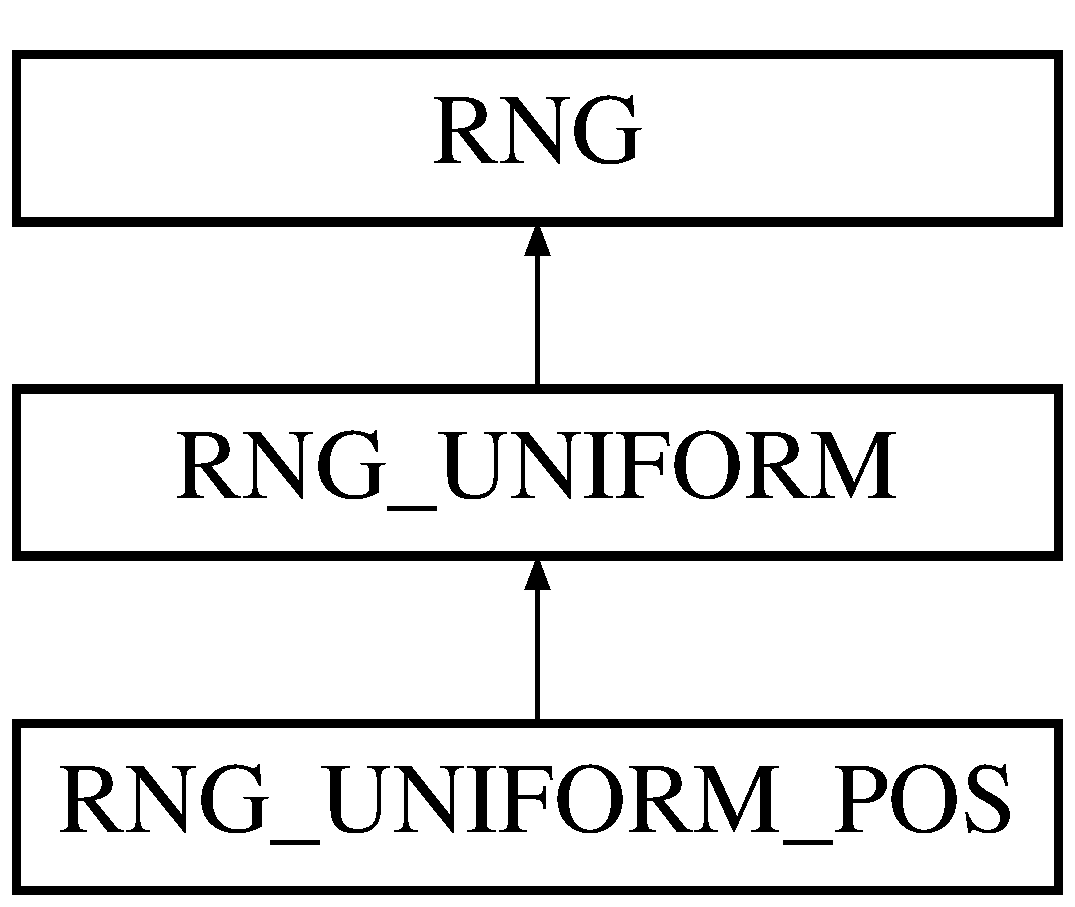
\includegraphics[height=3cm]{classRNG__UNIFORM__POS}
\end{center}
\end{figure}
\subsection*{Public Member Functions}
\begin{CompactItemize}
\item 
\textbf{RNG\_\-UNIFORM\_\-POS} (const gsl\_\-rng\_\-type $\ast$)\label{classRNG__UNIFORM__POS_ef9266ce4a054dde077bb95cfa548757}

\item 
\textbf{RNG\_\-UNIFORM\_\-POS} (const gsl\_\-rng\_\-type $\ast$, const unsigned long)\label{classRNG__UNIFORM__POS_809eebfa6a3bd38f18c3d9c4b9d29781}

\item 
virtual long double \textbf{Get} ()\label{classRNG__UNIFORM__POS_bf2efb204d4b2fed4664239ec15d9ea9}

\end{CompactItemize}


\subsection{Detailed Description}
\begin{Desc}
\item[Author:]Krishnan S \end{Desc}




The documentation for this class was generated from the following files:\begin{CompactItemize}
\item 
rng\_\-uniform\_\-pos.h\item 
rng\_\-uniform\_\-pos.cpp\end{CompactItemize}
